\documentclass{beamer}
\usepackage[utf8]{inputenc}
\usepackage{graphicx}
\usepackage[croatian]{babel}


\begin{document}

\maketitle

\section{Introduction}
\begin{frame}{TortoiseSVN}
\begin{itemize}
    \item Besplatan software
    \item Open source
    \item Lagan za korištenje
    \item Jednostavno i user-friendly sučelje
    \item Graf commitova
    \item Odlično integriran s Windowsom
    
    
\end{itemize}
    
\end{frame}
\begin{frame}{Spajanje u Tortoiseu}
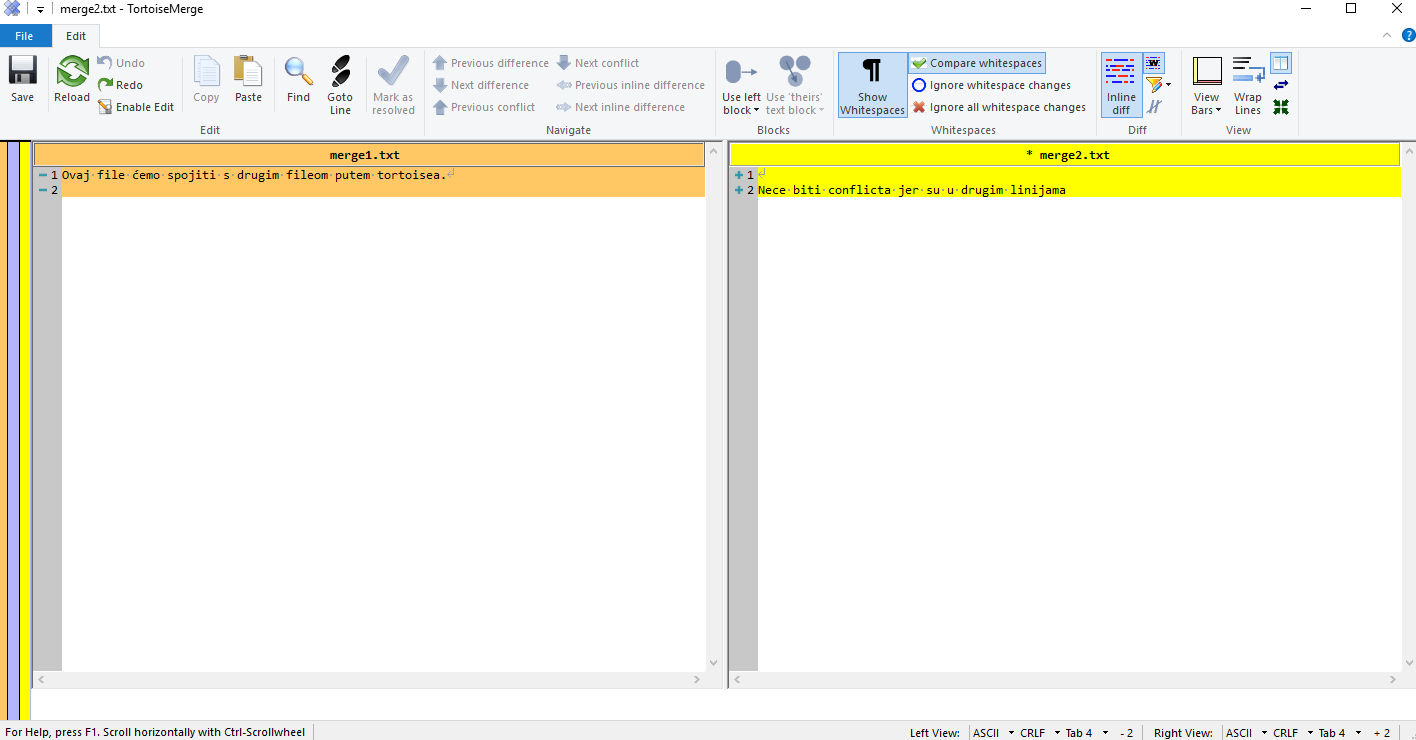
\includegraphics[width=10cm]{tortoise1.png}
\end{frame}
\begin{frame}
\begin{itemize}
    \item\small{Datoteka merge1 spojena u merge2}
\end{itemize}
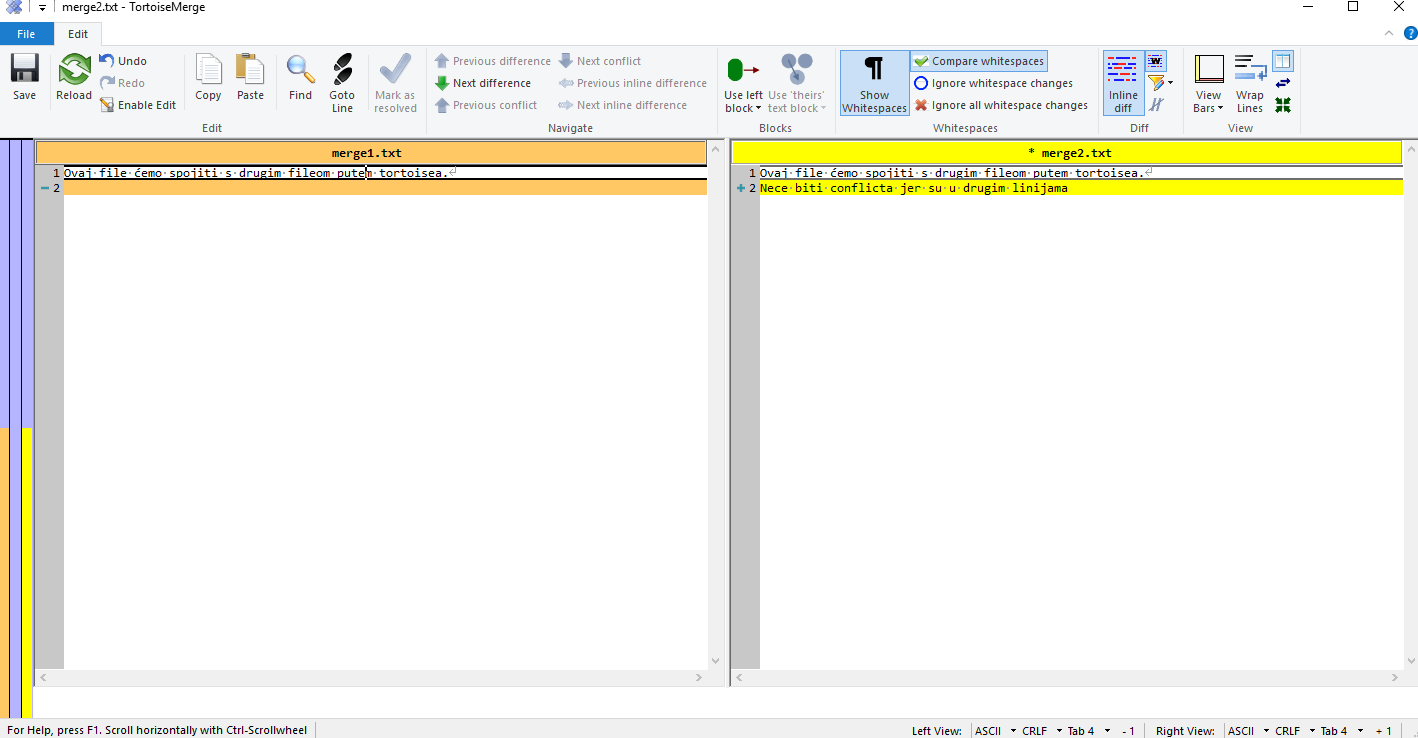
\includegraphics[height=4cm, width=10cm]{tortoise2.png}\newline
\begin{itemize}
    \item\small{Vidljivo kad otvorimo sami file}
\end{itemize}
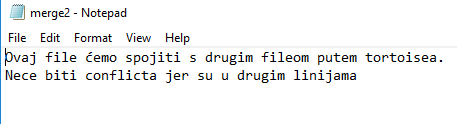
\includegraphics[width=7cm]{tortoise3.png}
\end{frame}

\end{document}
